\section {Power plane}

\begin{figure}
\centering
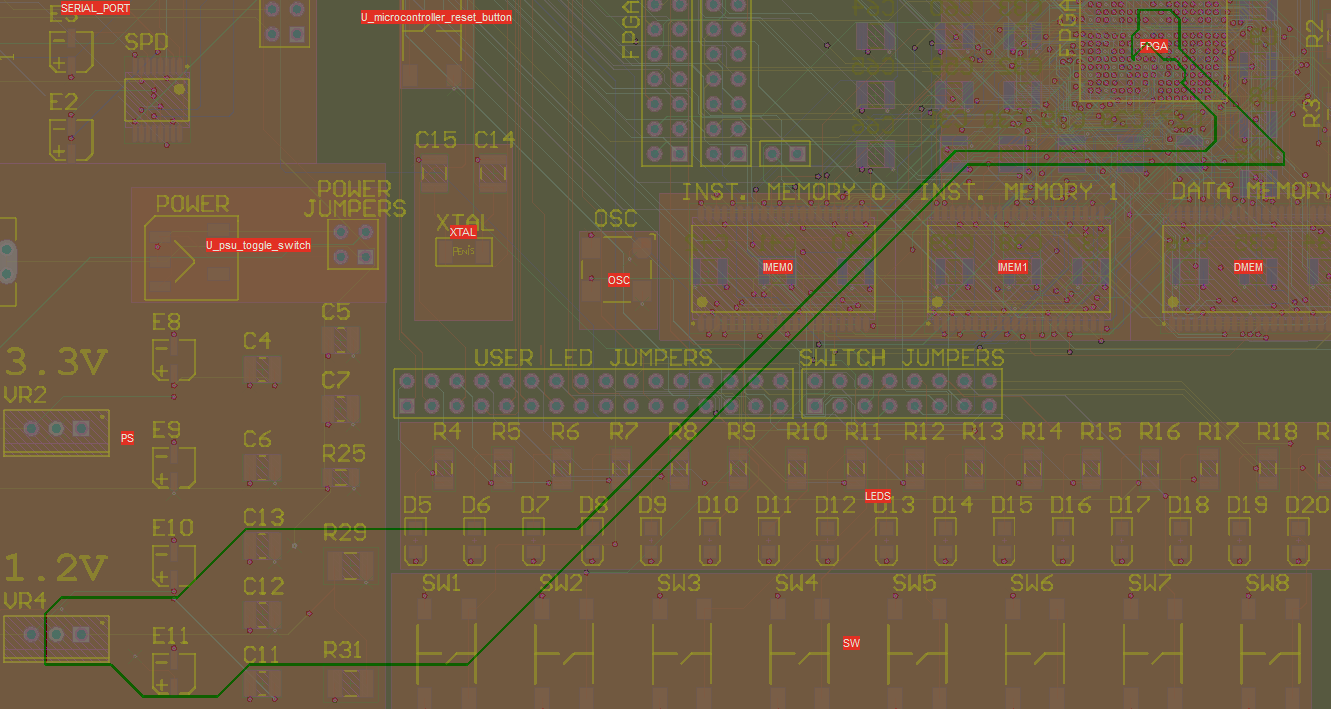
\includegraphics[width=10cm,keepaspectratio]{pcb/powerplanephoto.png}
\caption{Final design of the power plane. The power plane for 1.2V is the long polygon that goes from the ``powersupply'' part of the board to the FPGA core. The
design is also focusing on having as low path as possible to all the components that are using the power grid.  }
\label{figure:powerplanephoto}
\end{figure}

For simpler routing, reduced noise and to reduce voltage drop we have used power nets in this project.
As shown in above the pcb have a dedicated layer for power.
There is a wide track with 1.2 volts for the FPGA and the rest of the layer is one large 3.3 volt power net for all the other components.
In addition to these nets there is a dedicated layer for ground. The reason why we selected the design is done in this way is to provide as short routing path as possible for the sources using the power planes.
Keeping a short distance as possible on all signals is important in order to ensure as low loss of effect (measured in Watts) as possible.

